\documentclass{article}

\usepackage[margin=1in]{geometry}

% ToC
\usepackage{blindtext} 
\usepackage[linktocpage]{hyperref}
\usepackage{bookmark}
\usepackage{titlesec}

% bib
\usepackage[round]{natbib}

% Math Imports
\usepackage{amsmath, amssymb, bm, fancyhdr, sectsty, dsfont, mathtools}

% Tikz
\usepackage{tikz}
\usetikzlibrary{bayesnet}

\usepackage{wrapfig}
\usepackage{comment}
\usepackage{subcaption}

% Symbols
\newcommand\ind{\protect\mathpalette{\protect\independenT}{\perp}}
\def\independenT#1#2{\mathrel{\rlap{$#1#2$}\mkern2mu{#1#2}}}
\newcommand\norm[1]{\left\lVert#1\right\rVert}
\newcommand\set[1]{\left\{#1\right\}}

\newcommand\RNN{\mathrm{RNN}}
\newcommand\MLP{\mathrm{MLP}}
\newcommand\enc{\mathrm{enc}}
\newcommand\softmax{\mathrm{softmax}}

% Distributions
\newcommand{\Cat}{\mathrm{Cat}}
\newcommand\Expo{\mathrm{Expo}}
\newcommand\Bern{\mathrm{Bern}}
\newcommand\Pois{\mathrm{Pois}}
\newcommand\Bin{\mathrm{Bin}}
\newcommand\Unif{\mathrm{Unif}}
\newcommand\Betad{\mathrm{Beta}}
\newcommand\Gammad{\mathrm{Gamma}}
\newcommand\Geom{\mathrm{Geom}}
\newcommand\Logd{\mathrm{Logistic}}

\newcommand\E[1]{\mathbb{E}\left[#1\right]}
\newcommand\Es[2]{\mathbb{E}_{#1}\left[#2\right]}
\newcommand{\Var}{\mathrm{Var}}
\newcommand{\Cov}{\mathrm{Cov}}
\newcommand{\Cor}{\mathrm{Cor}}

% Bold stuff
\newcommand{\ba}{\mathbf{a}}
\newcommand{\bb}{\mathbf{b}}
\newcommand{\bc}{\mathbf{c}}
\newcommand{\bd}{\mathbf{d}}
\newcommand{\be}{\mathbf{e}}
\newcommand{\bg}{\mathbf{g}}
\newcommand{\bh}{\mathbf{h}}
\newcommand{\bw}{\mathbf{w}}
\newcommand{\bx}{\mathbf{x}}
\newcommand{\by}{\mathbf{y}}
\newcommand{\bz}{\mathbf{z}}

% mathcal stuff
\newcommand{\mcD}{\mathcal{D}}

% math blackboard bold stuff
\newcommand{\R}{\mathbb{R}}
\newcommand{\C}{\mathbb{C}}
\newcommand{\Z}{\mathbb{Z}}
\newcommand{\N}{\mathbb{N}}
\newcommand{\Q}{\mathbb{Q}}


\DeclareMathOperator*{\argmin}{argmin}
\DeclareMathOperator*{\argmax}{argmax}

\title{Latent Data to Document}

\begin{document}
\maketitle

\section{Introduction}
Neural network-based language models have achieved top performance,
allowing text generation models to become proficient at
generating short snippets of fluent text.
%However, we do not .

Goals:
\begin{itemize}
\item No lying
\item Modularity?
\item Interpretability?
\item If we remove burden from the language model, will it lie less?
Only have the LM focus on fluency
\end{itemize}

\section{Problem}
We would like to learn a conditional model
over sentences $\by = \{y_0, y_1, \ldots\}$ and latent structure $\bz$
given a table $\bx$.
We are primarily interested in the respective conditional distributions:
both the posterior distribution over structure given a sentence and table $p(\bz\mid\by,\bx)$,
as well as the conditional distribution over summaries
$p(\by\mid\bx)=\Es{\bz\sim p(\bz\mid\bx)}{p(\by\mid\bz,\bx)}$.
Note that the posterior distribution over structure $p(\bz\mid\by,\bx)$
is an information extraction model.

\section{Data to Document}
The copy models in \citet{wiseman2017d2t} are trained independently from the information extraction model. 
The copy model is trained by generating the summary conditioned on the full table.
The information extraction model used for evaluation is trained using labels
created by comparing tokens in the summary with the entities and values from the database.
See \citet{wiseman2017d2t} for all the tricks used in training the model.

Our goal is to use more structure in our model in order to unburden the language model
and prevent hallucination of facts.

We assume that every sentence has an implicit labelling or cluster.


\subsection{The Model}
Let $y_t$ be the current token, $\by_{0:t-1}$ all previous tokens,

\begin{figure}[ht]
\centering
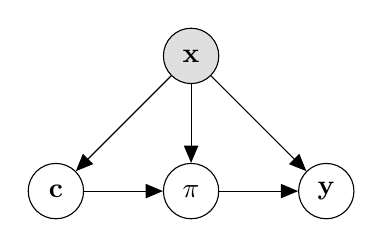
\begin{tikzpicture}
\node(x)[obs]{$\bx$};
\node(pi)[latent, below =of x]{$\pi$};
\node(c)[latent, left =of pi]{$\bc$};
\node(y)[latent, right =of pi]{$\by$};

\edge {x} {c};
\edge {x} {pi};
\edge {x} {y};
\edge {c} {pi};
\edge {pi} {y};

\end{tikzpicture}
\label{fig:dgm}
\caption{Directed graphical models for the two simplest latent variable models.
The observed context is $\tilde\bx$, current attention $a_t$, previous attention $a_{t-1}$,
state $s_t$, and target word $y_t$.}
\end{figure}

\section{Generative Model}
We decompose structure into content selection and ordering respectively:
$\bz = \set{\bc, \pi}$.
Actually, content selection might be bad and we may way to perform content selection and 
ordering jointly.
\begin{description}
\item[Content Selection]
$p(\bc\mid\bx)$ where $\bc\in\set{0,1}^n$ is a distribution over
binary masks over relations.
If a mask value is 1 then that specific relation is used to produce 
a summary.
\item[Content Ordering]
$p(\pi\mid\bc,\bx)$, where $\pi$ is a permutation matrix.
We may model this implicitly with a language model over relations, i.e. debagging.
Error: we may have repeated records.
It may be possible that certain records are only referred to a single time
while we should be available for use multiple times.
\item[Relation Realization]
$p(\by\mid\pi(\bc),\bx) = \prod_t p(y_t\mid\by_{<t}\pi(\bc)[t],\bx))$.
\end{description}

It may be better to simply 

\subsection{Information Extraction Model}
Recall the information extraction model from \citet{wiseman2017d2t}. $q$

\subsection{Learning Conjunctions}
Introduce latent variable $\bh$ and 

\subsection{Approximate Posterior or Posterior Regularization?}

\subsection{Noisy Channel?}
Introduce latent variable $\bh$ and 

\section{Training and Inference}
To start, we let $q(\bz\mid\\by,\bx)$ take the form of a
delta function take the form of a segmentation.
$$q(z_t\mid\by,\bx)=$$

\section{Related Work}

\section{Results}

\bibliographystyle{plainnat}
\bibliography{w}

\end{document}

